% TODO https://fidoalliance.org/specifications/
% TODO https://fidoalliance.org/overview/history/

\section{History and evolution}

The \wa{} is an outcome of joint efforts from the \gls{fido} alliance and and the \gls{w3c}. It is a product from various preceding industry standards, namely \gls{uaf} and \gls{u2f}. This chapter introduces the origin of the \wa{} by explaining the origin of the \gls{fido} alliance and their works on the \gls{uaf} and \gls{u2f} with a focus of the technical implementations, protocols and used techniques.

\subsection{FIDO Alliance}

The \gls{fido} alliance is an open industry association founded in July 2012 and launched in February 2013. Companies such as PayPal, Lenovo, and Infineon founded the \gls{fido} alliance. Currently the alliance has more than 260 members, including, e.g., Google, Amazon, Yubico, Samsung, Microsoft, VISA, or MasterCard. The goal of the \gls{fido} alliance is to develop new authentication protocols and standards in order to enhance and simplify the user experience of \gls{mfa} and to reduce the over usage of passwords.\footcites[See][583]{eckert-it-sec-9}

The \gls{fido} alliance developed the specifications \gls{uaf} and \gls{u2f}. The first specification of the \gls{u2f} was the starting point for the development of the \wa{} in a joint efforts with the \gls{w3c}. The \gls{ctap} is based on the \gls{u2f} specification 1.2 which complements the \wa. Both projects are part of the FIDO2 project.\footcite[See][169--170]{grimes2017hacking}

% TODO sources
\subsection{Universal Authentication Framework}

The \glsfirst{uaf} is \gls{fido}'s solution for a passwordless experience. It uses local and native device authentication, such as biometrics, to authorize the user. \gls{uaf} does not feature \gls{2fa} but is instead meant as a direct replacement for the login with passwords. It is based on public-key cryptography with the use of challenge-response authentication. The goal of the \gls{uaf} is to provide a generic \gls{api} that enables interoperability and unified user experience between the different operating systems and clients.

It features three key components, the \textit{\gls{uaf} client}, the \textit{\gls{uaf} server}, and the \textit{\gls{uaf} authenticators}. Besides that, the alliance offers a metadata service. The communication between the client and the authenticator is done via the \gls{uaf} \gls{asm}, which offers a standardized solution for the client to access and detect the different authenticators. Each authenticator is identified by the \gls{aaid}, a unique model ID that comprises the vendor and model ID, where the \gls{fido} alliance centrally assigns the vendor ID.

\begin{figure}[hbt]
	\centering
	\includegraphics[width=\textwidth]{pics/Picture1}
	\caption[\gls{uaf} architecture overview]{\gls{uaf} architecture overview\footnotemark}
	\label{fig:uaf_architecture}
\end{figure}
\footcitetext[Source: diagram by author, based on][4]{uaf-overview}

\autoref{fig:uaf_architecture} shows the \gls{uaf} architecture, where the client and user device are responsible for the communication between the authenticator, the \gls{fido} client and the corresponding web browser or (mobile) app, also called the user agent. The relying party, mostly a web server and \gls{fido} are responsible for secure communication of the \gls{uaf} protocol between the \gls{fido} client and server, as well as authenticator validation and user authentication. The metadata service updates the database of approved, genuine, and certificated authenticators that the server keeps. The protocol defines four different uses cases, which are explained in more detail below:

\begin{enumerate}
	\item registration of the authenticator
	\item user authentication
	\item transaction confirmation
	\item de-registration of the authenticator
\end{enumerate}

\subsubsection{Registration}

The registration process contains different steps. The \gls{fido} server generates a policy object which contains allowed and disallowed authenticators, and sends it together with the server challenge, username, the \textit{AppID}, and \textit{FacetID}, which are the origin of the server, to the client. The client checks that the given AppID matches the requested server and processes the registration. In the first place, the \gls{fcp} is generated by hashing the server challenge, AppID, FacetID, and \gls{tls} data. Subsequently, the \gls{asm} computes the \textit{KHAccessToken}, an access control mechanism to prevent unauthorized access to the authenticator. It comprises the AppID, ASMToken (a randomly generated and maintained secret by the \gls{asm}), PersonalID (a unique ID for each \gls{os} user account), and the CallerID (the assigned ID of the \gls{os} for the \gls{fido} client).

Once the \gls{fcp} and KHAccessToken are generated, the client sends the hashed \gls{fcp}, KHAccessToken, and username to the authenticator. After receiving the data, the authenticator presents the data to the user (e.g., the AppID in a display) and asks for user verification. When the user has been verified, and they approved the request, the authenticator generates a new key-pair and stores the data as the key handle in its secure storage. The key handle consists of the private key, KHAccessToken hash, and username. The key handle might be wrapped, i.e., encrypted in a way that only the client, \gls{asm} and authenticator can decrypt it again. It as to be noted though, that the exact generation of the key handle is explicitly not specified, i.e., it varies among the vendors of \gls{uaf} authenticators.

 After that, a \gls{krd} object is sent back to the client. It contains the \gls{aaid}, a signature counter, a registration counter, the hashed \gls{fcp}, the public key, the key handle, and the attestation certificate of the authenticator. Further, a signature over the values \gls{aaid}, hashed \gls{fcp}, counters, and the public key is signed by the private attestation key of the authenticator.

Finally, when the \gls{fido} server receives the registration request (\gls{krd} and signature) back, it can cryptographically verify the data by checking the sent signature, the attestation certificate, the \gls{aaid} of the authenticator and the hash of the \gls{fcp}. Ultimately, the server stores the public key in the database.

\footcites[See][191]{7897543}[See][131]{10.1007/978-3-319-67639-5_11}[See][]{uaf-asm}

\subsubsection{Authentication}

The authentication process is similar to the registration flow. When a user initiates the authentication, the relying party sends the same data as before, the policy, AppID, and challenge. The \gls{fido} client again determines the correct authenticator based on the received server policy and the sent AppID. The \gls{fcp} and its hash are generated in the same way as in the registration process. Further, the key handle and KHAccessToken are retrieved from the database and sent to the authenticator.

When the authenticator receives the key handle and KHAccessToken and the hash of the \gls{fcp}, this data is again verified. If it matches, the user has been verified, and they approved the authentication request, the corresponding private key is retrieved from the key handle and the signature counter increased. The authenticator sends the hashed \gls{fcp}, the counter and a \gls{nonce}, as well as a signature signed by the private key consisting of the hashed \gls{fcp}, nonce, and counter, back to the client which in turn sends the data to the relying party. Finally, the relying party can cryptographically verify the sent data by the signature and proceed with the authentication.

\subsubsection{Transaction Confirmation}

Confirming the transaction is a special use case of the authentication process. The same mechanisms and security features are used, and the only difference is the additional transaction text the \gls{fido} server sends to the client and which is in return displayed on display from the authenticator. This feature enables the \gls{uaf} protocol to not only authenticate a user but also to let the user confirm certain transactions. The specifications list the authenticator display as optional. In this case, the \gls{asm} can offer the display functions as a software solution.

\subsubsection{De-registration}

In contrast to the authentication and registration process, the de-registration process of authenticators is done without user verification. The server or client can initiate the process. The necessary information that the \gls{fido} client and \gls{asm} send to the authenticator is the AppID and optionally the specific credential, identified by the KeyID. To ensure the genuineness of the request, the client checks that the AppID matches the origin of the request.

% TODO sources
\subsection{Universal Second Factor}

The \glsfirst{u2f} is the second open standard developed by the \gls{fido} alliance prior to the \wa. It explicitly defines the use of a second factor, which is backed by public-key cryptography, for the password-based login flow. The main contributors are Google and Yubico, both being alliance members. The \textit{strong second factor} can be either connected or disconnected, e.g, built in hardware or for instance an \gls{usb} token, \gls{nfc}-capable device, or a standalone \gls{ble} dongle. The protocol defines two layers:

\begin{enumerate}
	\item the first layer defines the cryptographic basics of the protocol
	\item the second layer defines the communication between the user's authenticator and the first layer over the chosen transport protocol (such as \gls{usb}, \gls{nfc}, or \gls{ble})
\end{enumerate}

Besides that, the \gls{u2f} protocol only specifies \gls{usb}-\gls{hid} devices (internal or external), \gls{nfc}, Bluetooth, and the low energy variant \gls{ble}, as possible transport protocols.

The \gls{u2f} protocol relies on a web browser that is \gls{u2f}-capable and a web server that supports \gls{u2f} protocol and the authenticator, called the \gls{u2f} token. Two different operations are defined by the specification, the \textit{registration} and \textit{authentication} by generating a signature, both are explained in more detailed below.

Because it relies on the web in contrast to the \gls{uaf} protocol, browser support has to be taken into account. Due to the fact, that \gls{u2f} is superseded by \gls{fido}2, the browser support of \gls{u2f} is not of interest for this thesis.

Moreover, \gls{u2f} has also been renamed to \gls{ctap}1 since the release of the \gls{fido}2 to avoid confusion and questions whether \gls{u2f} can be used for the \wa{} as the \gls{ctap} protocol. However, a crucial restriction of the legacy \gls{u2f} protocol in usage with \gls{fido}2 is, that it is only usable as a second factor and not for passwordless logins.

\subsubsection{Registration}

\begin{figure}[hbt]
	\centering
	\includegraphics[width=\textwidth]{pics/u2f_reg}
	\caption[\gls{u2f} registration process]{\gls{u2f} registration process\footnotemark}
	\label{fig:u2f_reg}
\end{figure}
\footnotetext{source:...}

A requirement of the registration process of a \gls{u2f} token is that the user already is registered by the relying party, the web server. The registration process is similar to the introduced process of the \gls{uaf} protocol and also displayed in \autoref{fig:u2f_reg}. At first, the server generates a challenge for the client and sends it along with the username and it's AppID to the client, in this case the web browser. The payload also contains the desired version of the \gls{u2f} protocol and the already registered keys, if any. The client again can verify that the AppID matches the origin it is communicating with.

Further, the challenge parameters are constructed by hashing the challenge and AppID and sent along with the hash of the AppID to the \gls{u2f} token. After that, the token optionally verifies the presence of the user and generates a new public-private key pair over the \gls{nist} \gls{ec} P-256 and stores it with the username. The token sends the \textit{registration data} consisting of the public key, i.e. an uncompress point on the curve and the key handle, which can be wrapped, i.e., encrypted, back to the client. In addition, the attestation certificate of the token and an \gls{ecdsa} signature over the values: hashed AppID, hashed challenge, key handle, and pubic key are sent back to the client.

Finally, the client forwards the data to the relying party, which can cryptographically verify the data by the signature and attestation certificate.

The following \autoref{listing:u2f_reg} shows the high-level \gls{api} JavaScript registration process. 

\begin{example}{Example U2F registration code}
\begin{minted}[breaklines]{javascript}
const registerRequest = {
  challenge: 'Wings2019', // normally is a random string
  version: 'U2F_V2' // where V2 refers to protocol version 1.2
  appId: 'https://timbrust.de'
};

u2f.register('https://timbrust.de', [registerRequest], [], (response) => {
  console.log(response)
});
\end{minted}
\label{listing:u2f_reg}
\end{example}

The challenge value in the \textit{registerRequest} usually is a random challenge and base64 encoded, but for demonstration purposes a plain text string is used instead. In a real world scenario, the \textit{registerRequest} object is generated by the server and sent to the client and the \textit{u2f} JavaScript object is called from the client.

The received response is displayed in \autoref{listing:u2f_reg_resp} and contains the already explained bas64 encoded \textit{registrationData} and the base64 encoded \textit{clientData}. For better readability the strings clientData and registrationData are trimmed. Also, the clientData is decoded to show which data it contains.

\begin{example}{Example U2F registration response}
\begin{minted}[breaklines]{javascript}
const response = {
  clientData: 'eyJjaGFsbGVuZ2UiOiJXaW5nczIwMTkiLCJvcmlnaW4i [...]', // further data is omitted for readability
  errorCode: 0,
  registrationData: '...', // omitted for readability
  version: "U2F_V2"
}

// bota() decoded clientData yields
const decodedClientData = {
  challenge: 'Wings2019',
  origin: 'https://timbrust.de',
  typ: 'navigator.id.finishEnrollment'
}
\end{minted}
\label{listing:u2f_reg_resp}
\end{example}

The client always returns a \textit{type} with the value \textit{navigator.id.finishEnrollment} for a successful registration as well as the challenge of the relying party and its origin. The errorCode \textit{0 (OK)} indicates a successful registration. Other error codes include an other error (1), bad request (2), unsupported configuration (3), ineligible device (4), or timeout (5).

\subsubsection{Authentication}

\begin{figure}[hbt]
	\centering
	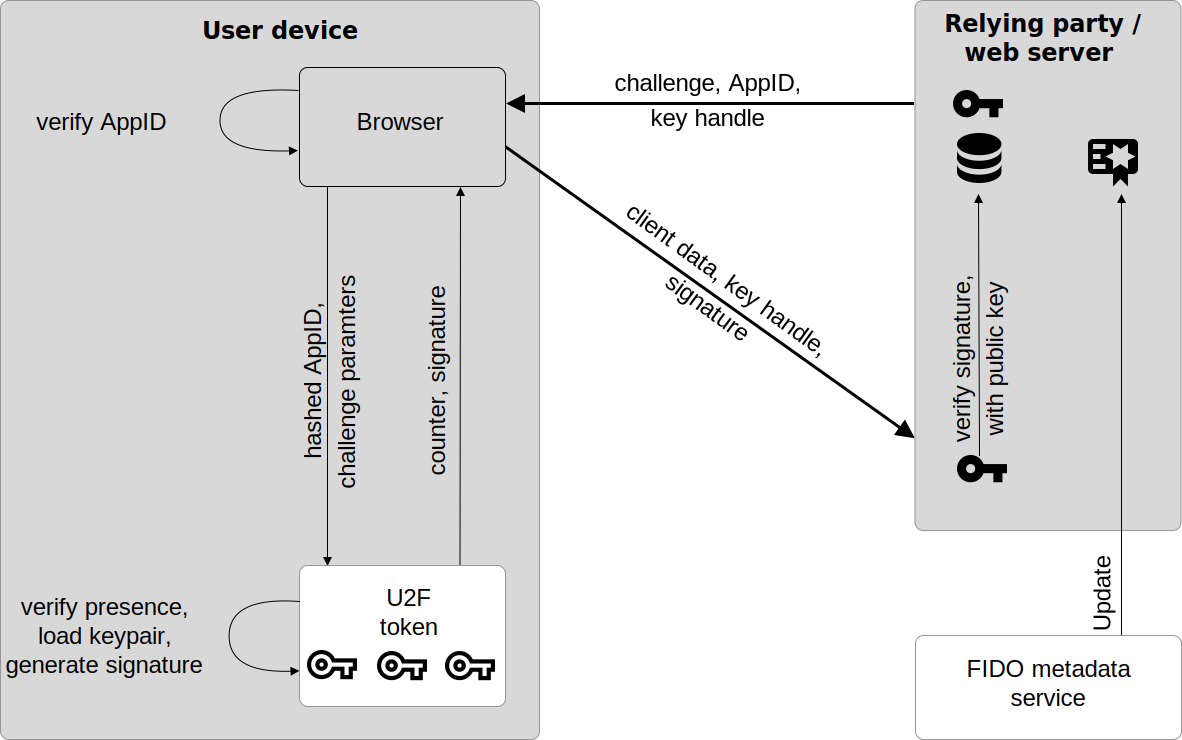
\includegraphics[width=\textwidth]{pics/u2f_auth}
	\caption[\gls{u2f} authentication process]{\gls{u2f} authenication process\footnotemark}
	\label{fig:u2f_auth}
\end{figure}
\footnotetext{source:...}

\begin{example}{Example U2F authentication code}
\begin{minted}[breaklines]{javascript}
const registeredKey = {
  keyHandle: '_WFf5BJ1dwtSCFzfWHoqKUhc9M3Hi0Tv58LAtPz0qM6B3A [...]", // further data is omitted for readability',
  version: 'U2F_V2'
}

u2f.sign('https://timbrust.de', 'Wings2019Auth', [registeredKey], [], (response) => {
    console.log(response)
  }
)
\end{minted}
\label{listing:u2f_auth}
\end{example}

\begin{example}{Example U2F authentication response}
\begin{minted}[breaklines]{javascript}
const response = {
  clientData: 'eyJjaGFsbGVuZ2UiOiJXaW5nczIwMTlBdXRoIiwib3JpZ2luIjoiaHR0cH [...]', // further data is omitted for readability
  errorCode: 0,
  keyHandle: 'WFf5BJ1dwtSCFzfWHoqKUhc9M3Hi0Tv58LAtPz0qM6B3A-iT [...]', // further data is omitted for readability
  signatureData: 'AQAAAhIwRQIhAK7xli8pV2cc8TKTOYMcdiz-ZuNVesSajp5S1kS [...]', // further data is omitted for readability
}

// bota() decoded clientData yields
const decodedClientData = {
  challenge: 'Wings2019Auth',
  origin: 'https://timbrust.de',
  typ: 'navigator.id.getAssertion'
}
\end{minted}
\label{listing:u2f_auth_resp}
\end{example}

\footcites[See][1--2, 4]{u2f-overview}[See][4]{u2f-js-api}

\subsection{FIDO2}

\begin{figure}[hbt]
	\centering
	\includegraphics[width=\textwidth]{pics/FIDO2-Graphic-v2}
	\caption[\gls{fido}2 architecture overview]{\gls{fido}2 architecture overview\footnotemark}
	\label{fig:fido2_architecture}
\end{figure}
\footcitetext[Source: https://fidoalliance.org/specifications/][4]{uaf-overview}


\subsubsection{Client to Authenticator Protocol 2}

\subsubsection{Web Authentication API}

The \wa{} is backwards compatible to the \gls{u2f} compatible, thus making every security token that is usable for \gls{u2f} compatible with the \wa, too.